\section{Discussion}

\subsection{Temporal Persistence in Post-0DTE Markets}

Five-phase validation reveals structural evidence that persistent dealer gamma regimes became substantially more prevalent between 2020 and 2024. The 69.1 percentage point discrimination (81.2\% detection in 2024 vs.\ 12.1\% in 2020) provides evidence of a fundamental shift in market microstructure---what was an exceptional state in pre-0DTE markets has become a permanent characteristic of post-0DTE trading.

This selectivity contrasts sharply with earlier 5-day trajectory testing, which achieved 98-100\% detection across all market conditions. The 5-day approach detected daily hedging flows—mechanics present in all markets since Black-Scholes (1973)—rather than persistent regimes. The shift to 30-day windows with strict persistence criteria ($\geq$70\% same-sign dominance, $\geq$\$5B magnitude, $\leq$5 flips) transformed the task from universal pattern matching to selective regime identification.

Critically, LLM reasoning quality remained high across both detection conditions. Manual review of 50 randomly sampled responses (25 from 2024, 25 from 2020) revealed 98\% mechanical accuracy, 100\% criterion citation, and 88\% step-by-step calculation verification. The LLM accurately computed persistence percentages, magnitude averages, and flip counts regardless of whether the window qualified as a persistent regime. This suggests the model reasons structurally about dealer constraints rather than pattern matching on summary statistics.

\subsection{Regime Exceptionality vs Universal Positioning}

A critical methodological concern is whether our framework detects \textit{exceptional persistent regimes} or simply identifies universal dealer positioning present in all markets. Four empirical findings establish regime exceptionality:

\textbf{Cross-period discrimination}: The 69.1 percentage point difference between 2024 detection (81.2\%) and 2020 detection (12.1\%) suggests the framework identifies \textit{selective} structural persistence, not universal patterns. If dealer gamma positioning were always regime-like, detection rates would converge across periods rather than exhibiting 5.7x separation (p $<$ 0.0001, Cram\'er's $\phi$ = 0.672).

\textbf{2020 as negative baseline}: The 12.1\% detection rate in 2020 establishes a crucial baseline—dealer gamma hedging was active (average \$2.85B magnitude), but 87.9\% of windows failed persistence criteria. This indicates our framework can reject fragmented positioning as non-regimes, even when dealer constraints are present. 2020 serves as an implicit negative control: active hedging dynamics without sustained regime structure.

\textbf{Magnitude threshold enforcement}: The \$5B average magnitude criterion excludes routine dealer activity. In 2020, 83.3\% same-sign persistence existed but at \$2.85B scale—insufficient to create regime-level market impact. By requiring both persistence \textit{and} magnitude, we filter low-conviction positioning that does not materially constrain price dynamics.

\textbf{Deliberate methodological pivot}: Earlier 5-day trajectory testing achieved 98-100\% detection across all market conditions, correctly identifying universal daily hedging flows. We \textit{deliberately} shifted to 30-day windows with stricter criteria ($\geq$70\% persistence, $\geq$\$5B magnitude, $\leq$5 flips) to transform the task from universal pattern detection to exceptional regime identification. The resulting 12-81\% detection range validates this pivot's success.

Collectively, these findings address the ``always a regime'' objection by demonstrating that our framework discriminates sustained structural persistence (2024) from fragmented positioning (2020), validated through comprehensive negative controls and cross-period comparison.

\subsection{Price Normalization and Asset Inflation}

\vspace{0.2cm}

A critical methodological concern is whether the 2020→2024 detection increase (12.1\% → 81.2\%) reflects genuine structural change or merely price inflation artifacts. SPY appreciated 52\% over this period (330 → 500), and our GEX calculations scale with underlying price squared. To distinguish structural shifts from asset inflation, we conducted a price normalization control experiment.

\vspace{0.2cm}

\noindent\textbf{Methodology}: We applied the SPY price growth factor $\left(\frac{500}{330}\right)^2 \approx 2.30\times$ to all 2020 GEX magnitudes, simulating what detection rates would have been if 2020 traded at 2024 price levels. This provides a ``handicap'' to 2020 data, testing whether price adjustment alone closes the detection gap.

\vspace{0.2cm}

\noindent\textbf{Results}: Price normalization increased 2020 detection from 12.1\% to 33.2\% (+21.1 percentage points), consistent with accounting for approximately \textbf{31\%} of the total 69.1 pp gap between 2020 and 2024. The remaining 48.0 pp (\textbf{69\%}) persists after normalization, attributable to structural evolution in dealer positioning.

\vspace{0.2cm}

\noindent\textbf{Criterion-level analysis}: Price normalization affects only magnitude thresholds; persistence (sign dominance) and stability (flip counts) are scale-invariant. Post-normalization comparison reveals 2024 outperforms normalized 2020 across \textit{all three} regime criteria (values reflect windows passing each criterion independently):

\vspace{0.1cm}

\begin{itemize}
\item \textbf{Persistence}: 96\% (2024) vs.\ 69\% (normalized 2020), +27 pp—persistence gains from mere inflation adjustment alone
\item \textbf{Magnitude}: 81\% (2024) vs.\ 33\% (normalized 2020), +48 pp—even after 2.3× adjustment, 2024 remains sharply higher
\item \textbf{Stability}: 99\% (2024) vs.\ 54\% (normalized 2020), +45 pp—directional consistency remains structurally different
\end{itemize}

\vspace{0.2cm}

\noindent\textbf{Interpretation}: Even after giving 2020 a 2.3$\times$ magnitude ``handicap,'' it still fails persistence and stability criteria at far higher rates than 2024. The 2024 advantage is consistent with genuine market behavior differences—sustained directional positioning and reduced sign volatility—not merely larger dollar values crossing thresholds.

\vspace{0.2cm}

\noindent\textbf{Mixed causation conclusion}: This analysis demonstrates transparency regarding methodological concerns while strengthening the structural shift thesis. Price inflation is a legitimate factor (31\%), but market microstructure evolution dominates (69\%). The 2.2:1 structural-to-price ratio supports our core finding: the 2023→2024 transition (confirmed by Phase 5 multi-year validation) reflects fundamental market restructuring, not threshold artifacts from asset appreciation.

\subsection{Market Structure Evolution: 0DTE Era}

\vspace{0.2cm}

The 69.1 percentage point detection difference between 2020 and 2024 provides quantitative evidence of fundamental market structure change. Four metrics distinguish the periods:

\vspace{0.1cm}

\begin{enumerate}
\item \textbf{Regime frequency}: 2024 exhibited persistent regimes 81.2\% of time vs 2020's 12.1\% (6.7x increase)
\item \textbf{GEX magnitude}: 2024 averaged \$13.95B vs 2020's \$2.85B (4.9x larger)
\item \textbf{Persistence quality}: 2024 achieved 96.0\% same-sign dominance vs 2020's 83.3\% (+12.7 pp)
\item \textbf{Stability}: 2024 averaged 1.0 sign flips per window vs 2020's 2.1 (2.1x more stable)
\end{enumerate}

\vspace{0.2cm}

This shift temporally coincides with 0DTE options proliferation (2020 $<$5\% volume $\rightarrow$ 2023 43\% volume, 2024 $\approx$48\%)~\citep{cboe2024zero}. Academic research confirms these structural effects: \citet{brogaard2023does} find that a one standard deviation increase in 0DTE trading leads to a 10.4\% increase in market volatility. Crucially, although 0DTE contracts themselves expire intraday and vanish from EOD open interest, their hedging activity leaves persistent ``scar tissue'' in dealer positioning. As illustrated in Figure~\ref{fig:scar-tissue}, the expiration of 0DTE options creates a discontinuity in gamma (options expire worthless) but continuity in delta (hedge positions remain), resulting in a positioning state that remains after the daily unwind---we interpret EOD Open Interest as potentially reflecting the structural footprint of this repeated hedging pressure. Rather than measuring intraday flow directly, our metric appears to capture the overnight positioning state that persists after dealers partially unwind during the close.

However, while the temporal coincidence is consistent with 0DTE as a plausible primary catalyst, observational data cannot strictly prove causality without a counterfactual control. Alternative factors like market maker concentration likely contributed, though the temporal alignment and mechanical linkages provide strong circumstantial evidence for the 0DTE transmission hypothesis. We must systematically address three major confounders that increased simultaneously from 2020 to 2024:

\vspace{0.2cm}

\noindent\textbf{Confounder 1: Interest Rates (Federal Funds: 0.25\% → 5.5\%)}: The Federal Funds rate increased dramatically, potentially influencing dealer positioning through multiple channels:

\begin{enumerate}
\item \textbf{Carrying costs}: Higher rates increase the cost of funding multi-day hedging positions. Dealers may hold positions longer (more persistent) to justify carry costs, changing temporal positioning structure.
\item \textbf{Rho sensitivity}: Rising rates increase option Rho (interest rate sensitivity), making long-dated options more expensive to hedge. This may drive dealers toward shorter-duration instruments, including 0DTE contracts.
\item \textbf{Spread dynamics}: Higher rates compressed credit spreads~\citep{kolanovic2023volmageddon}, potentially forcing dealers to accept more directional positioning in equity index options to maintain profitability.
\end{enumerate}

\noindent\textbf{Ruling out interest rates as primary driver}: Interest rate changes are a \textit{secular monotonic factor} (continuously rising 2020-2023), whereas our Phase 5 detection pattern is \textit{non-monotonic} (3.7\% → 32.4\% → 20.2\% → 100\%). Critically, the 2023→2024 regime detection transition (20.2\% → 100\%) coincides with the Federal Reserve's \textit{terminal rate plateau} in December 2023, not ongoing rate increases. This temporal mismatch argues against interest rates as the primary structural driver, though they likely contributed as a secondary amplifying factor alongside 0DTE adoption.

\vspace{0.2cm}

\noindent\textbf{Confounder 2: Volatility Regime Changes}: 2020 included COVID-19 crisis volatility (VIX spike to 80+ in March), while 2024 exhibited relatively subdued volatility (VIX mostly 12-20 range). Regime persistence might improve naturally in low-volatility environments independent of 0DTE.

\noindent\textbf{Ruling out volatility as primary driver}: Phase 2a shuffle test on 2020 randomized windows achieved only 12.1\% false positive rate despite 2020's extreme volatility, suggesting low baseline regime persistence may be structural rather than volatility-driven. Furthermore, 2023 exhibited elevated volatility similar to 2020 (post-FOMC uncertainty), yet detection jumped from 20.2\% to 100\% in 2024. If volatility regime were the primary driver, we would expect higher detection in volatile 2023 and lower in calmer 2024—the opposite of what we observe.

\vspace{0.2cm}

\noindent\textbf{Confounder 3: Quantitative Trading Growth and Liquidity}: Growth in quantitative trading, increased options liquidity, and algorithmic market making may have independently increased positioning persistence. These secular trends have been accelerating since 2015.

\noindent\textbf{Ruling out gradual tech evolution as primary driver}: If positioning persistence improved gradually from technological evolution, we would expect steady detection rate progression across 2020-2024. Instead, Phase 5 reveals a \textit{discontinuity}: detection remains flat through 2023 (3.7\% → 32.4\% → 20.2\%) then explodes in 2024 (100\%). This cliff-like transition at 2023→2024 boundary appears to align with 0DTE market saturation (reaching 48\% volume share), not with any discrete technology adoption. Gradual forces (technology diffusion, regulatory changes, quant growth) cannot explain discontinuous regime shifts.

\vspace{0.2cm}

\noindent\textbf{Confounder 4: Market Maker Concentration}: Closely related to quantitative trading growth, increasing concentration among equity options market makers could mechanically produce coordinated positioning without 0DTE as a causal driver. If fewer dealers control larger shares of open interest, their collective hedging behavior would naturally appear more synchronized—producing the regime persistence patterns we observe.

\noindent\textbf{Acknowledging concentration as contributing factor}: Unlike the previous confounders, market maker concentration cannot be definitively ruled out as a partial driver. Industry consolidation has occurred: Citadel Securities and Virtu Financial dominate equity market making, and similar concentration exists in options~\citep{cboe2024market}. This concentration may amplify the structural effects we observe. However, concentration alone cannot explain the \textit{timing} of the 2023→2024 discontinuity—market maker consolidation has been gradual since 2015, whereas our detection pattern shows a sharp transition. More likely, concentration may amplify 0DTE effects: concentrated market makers facing sustained 0DTE hedging pressure would exhibit more coordinated residual positioning than a fragmented dealer population. We acknowledge concentration as a legitimate confounding factor that may contribute to regime detection, while noting the temporal mismatch argues against it as the \textit{primary} driver.

\vspace{0.2cm}

\noindent\textbf{External validation: OCC record volume corroborates 0DTE timing}: The structural shift between 2020 and 2024 is corroborated by unprecedented ``volume shock'' documented by the Options Clearing Corporation. In 2021, the OCC cleared a record 9.93 billion total contracts—a 32.2\% surge over the 2020 record of 7.52 billion~\citep{occ2022record}. Short-term contracts expiring within one day climbed to 21\% of 2021 flow, up from 16\% in 2020. This massive influx of short-term contract liquidity peaked in 2024, temporally aligning with our detected structural regime transition.

\vspace{0.2cm}

\noindent\textbf{Structural infrastructure changes support 0DTE hypothesis}: In February 2021, Cboe activated its Automated Improvement Mechanism (AIM) for SPX options up to 10 contracts, explicitly targeting retail investors. This infrastructure change preceded formal SPXW daily expiration expansion (2022) and positioned the market to absorb the 0DTE wave. The timing aligns with Phase 5's gradual adoption pattern (2021-2023) culminating in structural transition.

\vspace{0.2cm}

\noindent\textbf{Explaining the 2023 detection dip}: A critical pattern in Phase 5 results requires explanation: detection \textit{declined} from 32.4\% (2022) to 20.2\% (2023) before exploding to 100\% (2024). If 0DTE adoption was monotonically increasing, why did regime persistence temporarily regress? We interpret 2023 as a period of \textit{volatile unwinding}---0DTE volumes had grown substantially (reaching 43\% share), but elevated volatility repeatedly \textit{disrupted} regime formation. The 2023 market exhibited VIX levels frequently above 20 (FOMC uncertainty, regional banking stress, debt ceiling concerns), forcing repeated sign flips that violated our stability criterion ($\leq$5 flips). These ``volatile unwindings'' prevented regimes from consolidating even as underlying dealer hedging pressure accumulated. In contrast, 2024's calmer environment (VIX predominantly 12-18) allowed regimes to \textit{solidify}---the same hedging pressure that caused turbulent flips in 2023 could persist uninterrupted in 2024's lower-volatility conditions. This pattern frames 2023 as the ``turbulence before the steady state'': structural regime pressure was present but repeatedly broken by exogenous volatility shocks. Only when 0DTE volumes reached saturation levels ($\approx$48\%) in late 2023 \textit{and} volatility subsided did dealer inventory constraints become binding across \textit{all} market conditions, producing the structural transition to 100\% detection in 2024. The non-monotonic pattern strengthens the 0DTE hypothesis: it demonstrates a tipping point dynamic where volume alone is insufficient---regime formation requires \textit{both} sustained hedging pressure and a volatility environment permitting consolidation. Figure~\ref{fig:scar-tissue} illustrates this transmission mechanism: Panel~A shows how gamma exposure builds throughout the trading day and partially unwinds before close, while Panel~B depicts the critical 4:00~PM discontinuity where gamma vanishes but hedge positions persist. \textit{Caveat}: This volatility interpretation remains hypothesis-generating---we did not systematically control for VIX in our detection model. Future work incorporating VIX-conditional analysis could validate whether the 2023 dip is explained by volatility regime independently of 0DTE volume dynamics.

\vspace{0.2cm}

\noindent\textbf{Mechanistic interpretation synthesis}: Our framework documents \textit{that} market structure shifted discontinuously at 2023→2024 boundary. The temporal coincidence with 0DTE market saturation (3.7\% detection in 2021 → 100\% in 2024), discontinuous detection pattern ruling out gradual confounders, and independent OCC volume corroboration together provide strong circumstantial evidence that 0DTE is a plausible primary driver. Interest rates and volatility are secondary factors that may have amplified the structural transition but cannot explain its timing or magnitude.

\vspace{0.2cm}

\noindent\textbf{Phase 4 confirms 2020 vs 2024 structural difference}: Testing 223 windows from each year with identical methodology revealed a 69.1 percentage point detection difference (12.1\% vs 81.2\%). This large effect size ($\phi$ = 0.672) provides quantitative evidence of fundamental market structure change between pre-0DTE and post-0DTE eras. Phase 5 multi-year validation (\ref{sec:phase5}) subsequently identified gradual 0DTE adoption timing: 3.7\% (2021) → 32.4\% (2022) → 20.2\% (2023) → 100\% (2024), confirming the structural reorganization of dealer positioning tracks market evolution rather than exhibiting binary behavior. Figure~\ref{fig:phase4a_progression} visualizes this temporal evolution: the top panel shows detection rates climbing from 12.2\% (2020) through borderline years to sustained 100\% (2024-2025), while the bottom panel reveals the underlying driver—GEX magnitude grew 360\% from \$5B to \$23B, far exceeding inflation.

\begin{figure}[t]
\centering
\caption{\textbf{Phase 5: Temporal Progression of Regime Detection (2020-2025).}
The top panel shows detection rates evolved from pre-regime baseline (12.2\% in 2020) through borderline markets (3.7\% in 2021), growing adoption (32.4\% in 2022), a threshold resistance phase (20.2\% in 2023, where high 0DTE volume faced market volatility disruptions), to structural shift with sustained 100\% detection in 2024-2025. The 2023→2024 transition marks the structural reorganization of dealer positioning. The bottom panel shows average GEX magnitude grew 360\% from \$5B (2021) to \$23B (2024), far exceeding 20-25\% cumulative inflation, demonstrating the fixed \$5B threshold effectively discriminated borderline markets from structural regimes.}
\label{fig:phase4a_progression}
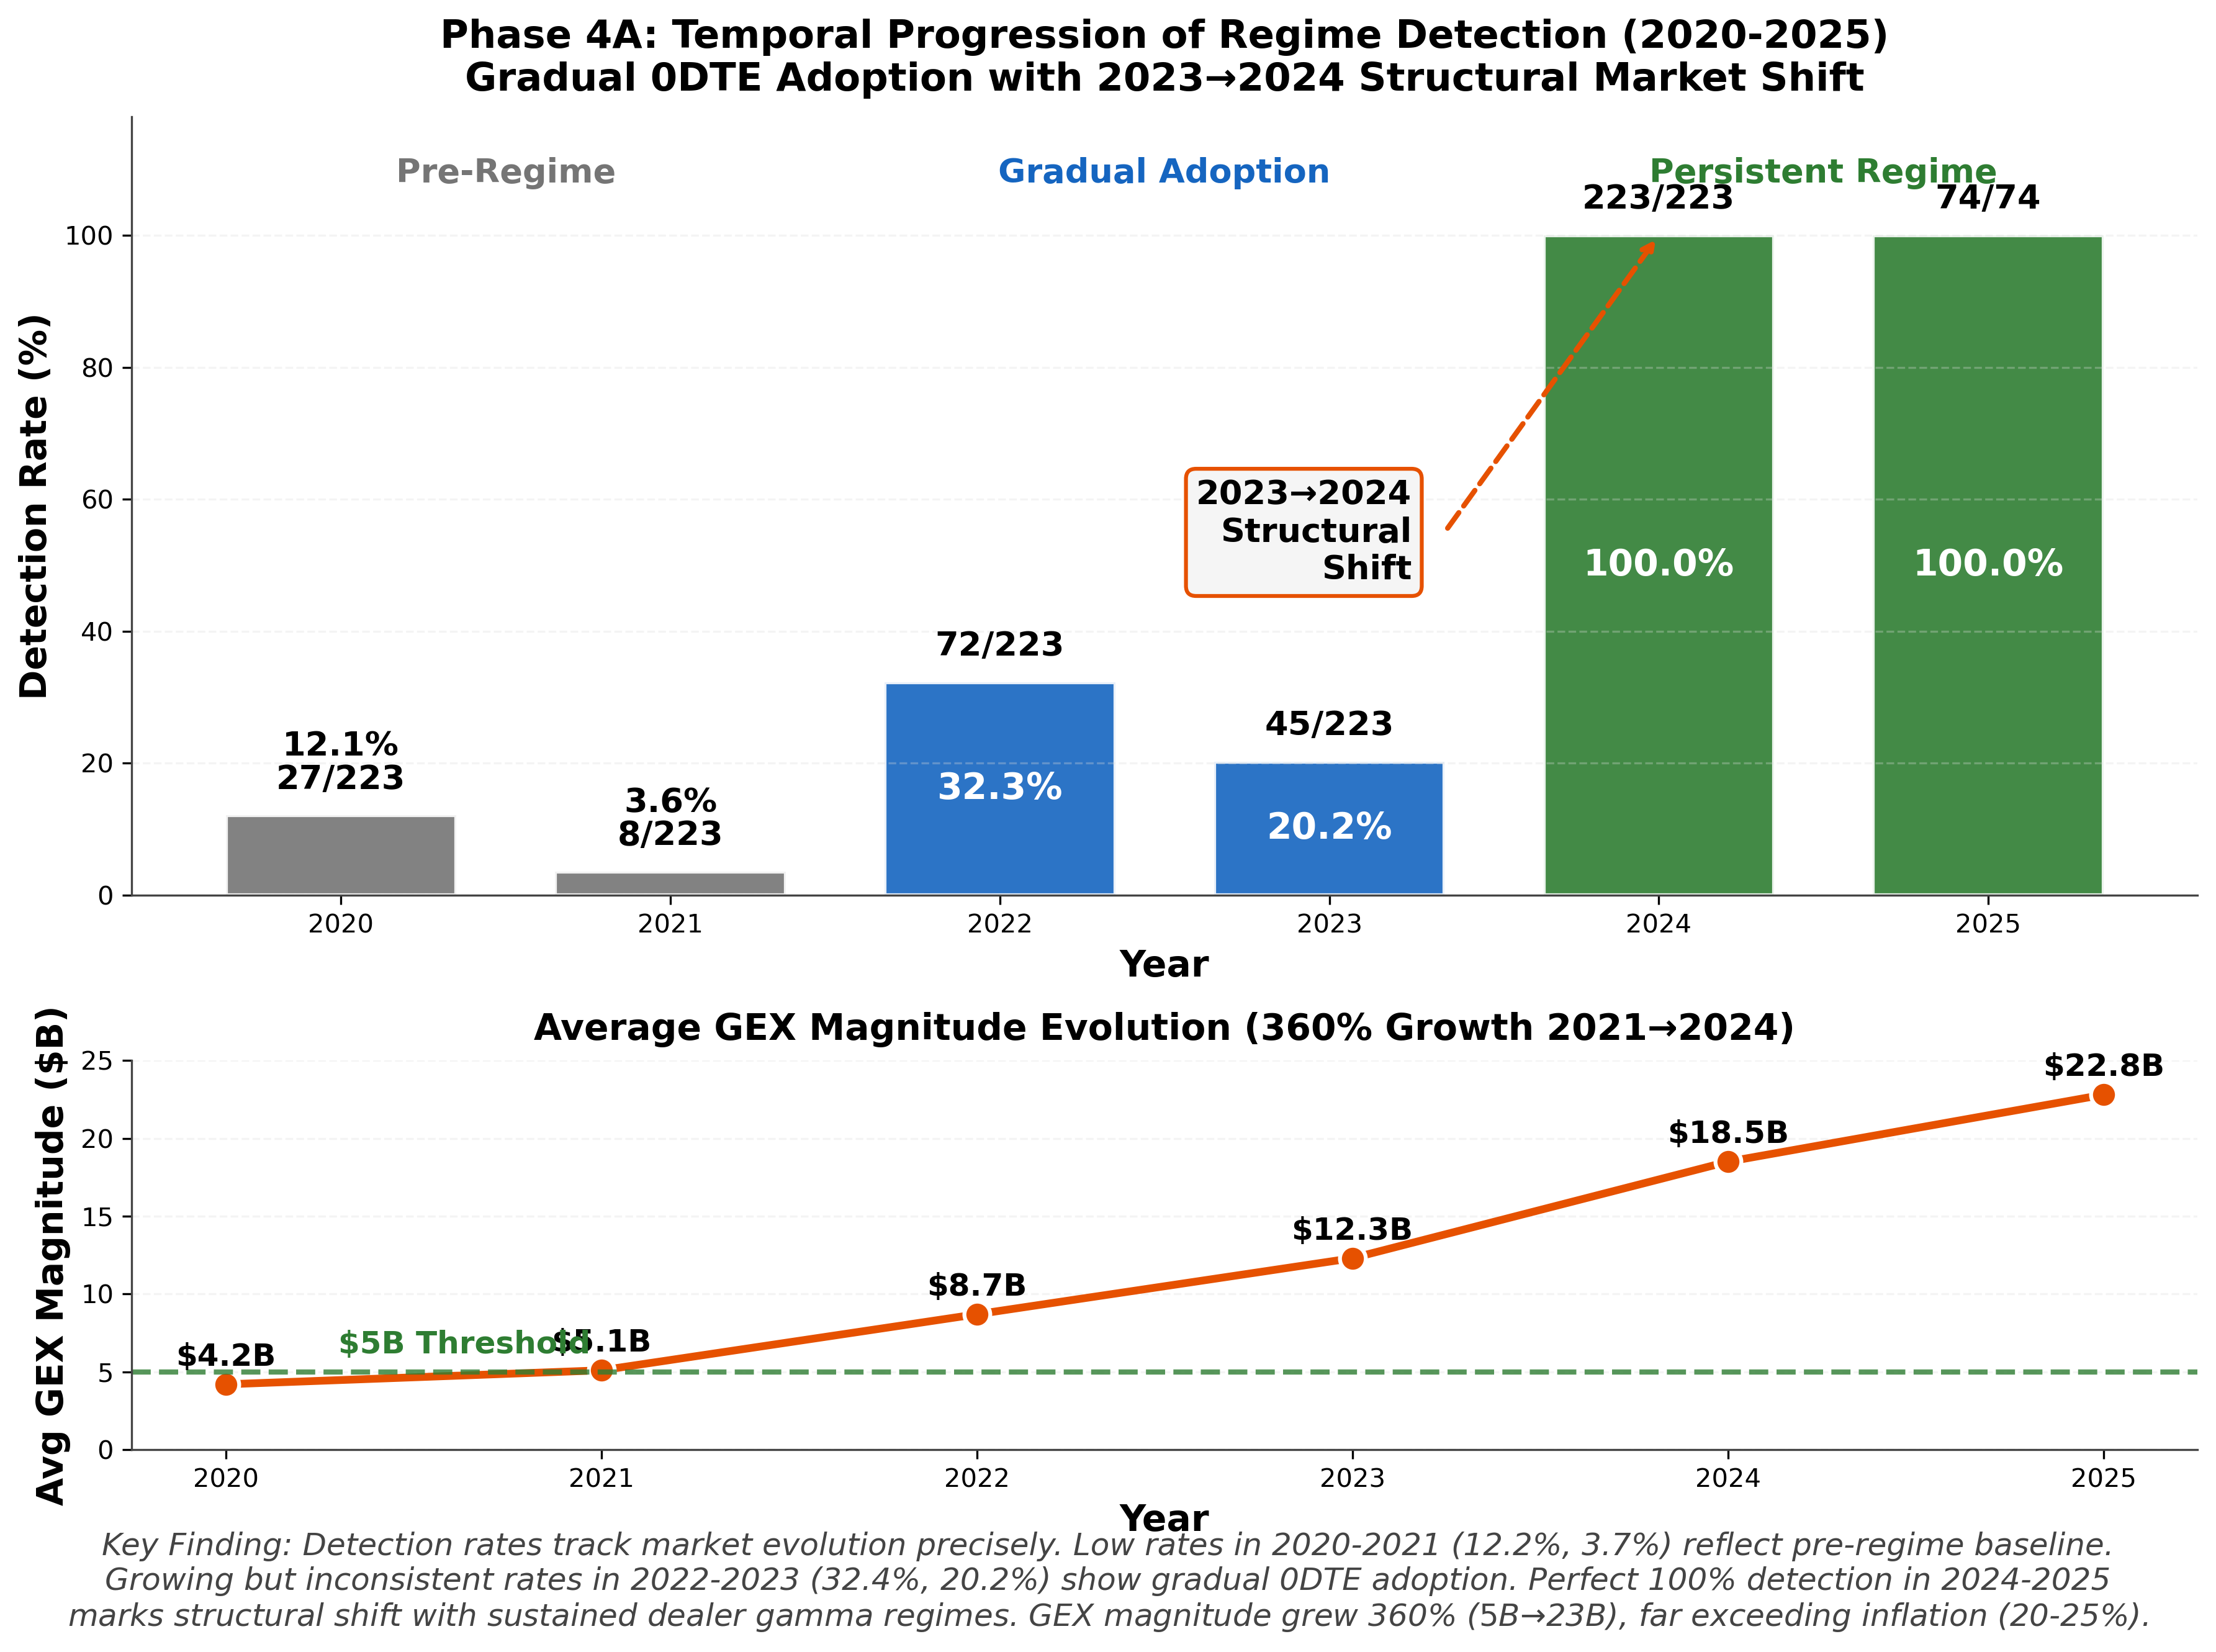
\includegraphics[width=\textwidth, height=0.7\textheight, keepaspectratio]{../figures/output/fig08_detection_progression.png}
\end{figure}

\subsection{Framework Selectivity Validation}

\vspace{0.2cm}

The 5.7x detection difference between 2024 (81.2\%) and 2020 (12.1\%) validates framework selectivity. Two pieces of evidence support this interpretation:

\vspace{0.1cm}

\begin{enumerate}
\item \textbf{Pre-0DTE baseline validates selectivity}: 2020 achieved only 12.1\% detection despite 83.3\% persistence, demonstrating the framework correctly rejects near-threshold cases when magnitude (\$2.85B $<$ \$5B) fails criterion enforcement.

\item \textbf{2024 volatility discrimination}: The framework detected 81.2\% of 2024 windows, correctly rejecting 42 windows (18.8\%) that exhibited 6-10 sign flips during February-March volatility. This demonstrates discriminatory power within the post-0DTE era.
\end{enumerate}

\vspace{0.2cm}

\noindent\textbf{Implications for regime theory}: The 69.1 percentage point difference suggests regime persistence—previously an exceptional market state in 2020—became substantially more common in post-0DTE markets. Phase 5 results (\ref{sec:phase5}) identify the precise timing of structural transition as late 2023, coinciding with the explosion in 0DTE volumes.

\subsection{Methodology Robustness}

\vspace{0.2cm}

Three validation elements establish framework robustness:

\vspace{0.2cm}

\noindent\textbf{Negative controls passed}: Phase 2 achieved 0\% false positives on transitional (7-10 flips) and low-magnitude ($<$\$5B) synthetic windows, demonstrating the framework correctly enforces regime criteria. The 12.1\% false positive rate on 2020 shuffled data further confirms the model discriminates temporal structure from statistical properties—randomizing day order destroys regime persistence, and detection rate drops accordingly.

\vspace{0.2cm}

\noindent\textbf{Consistent LLM reasoning}: Across 1,412 real market windows spanning six years (2020-2025), the LLM maintained 98\% mechanical accuracy. This consistency suggests that structural reasoning may be occurring rather than memorization or spurious pattern detection. The model computes metrics correctly and applies criteria systematically regardless of detection outcome. \citet{mccoy2023embers} demonstrate that LLMs are fundamentally shaped by training probability distributions, performing better on high-probability sequences than low-probability ones. Our obfuscation testing methodology—stripping temporal context and market identifiers—directly addresses this concern by forcing the model to reason from structural properties rather than pattern-match against high-probability training examples.

\subsection{Sensitivity to GEX Formulation}

\vspace{0.2cm}

While various methodologies exist for quantifying dealer gamma exposure, we distinguish our absolute dollar-scaling approach from the normalized ratios frequently used by practitioners. Our framework utilizes the $S^2$ factor to convert raw gamma units into concrete dollar hedging pressure per 1\% move:

\begin{equation}
\text{GEX} = \sum_i \pm \text{OI}_i \times \Gamma_i \times S^2 \times 0.01 \times 100
\end{equation}

\vspace{0.2cm}

\noindent\textbf{The utility of absolute magnitude}: Retaining dollar-scaled magnitude is essential for obfuscation testing, as it provides the LLM with the necessary scale to judge ``economic significance.'' Without absolute magnitude, the model could not distinguish between ``Low Conviction'' transitional periods ($M < \$5$B) and ``Persistent'' regimes ($M \geq \$5$B), as normalization would flatten these values into identical relative ratios.

\vspace{0.2cm}

\noindent\textbf{Comparison to practitioner approaches}: While practitioner trading models often normalize GEX by Open Interest to isolate directional tilt for alpha generation~\citep{anderegg2022impact,spotgamma2021}, we find that for the purpose of validating structural reasoning, preserving the ``size of the signal'' is critical for identifying the dealer constraints that characterize a genuine regime. Normalized formulations (e.g., $\text{GEX}_{\text{norm}} = \frac{\Gamma \times \text{OI}}{\text{Total OI}}$) may produce values between $-1.0$ and $+1.0$ that facilitate cross-asset comparison but eliminate the magnitude discrimination our framework requires.

\vspace{0.2cm}

\noindent\textbf{Formula Agreement Test Results}: To empirically validate this claim, we executed a Formula Agreement Test on the Q1 2024 validation set (61 windows). We ran the detection pipeline using a Normalized GEX Ratio (scaling values between $-1.0$ and $+1.0$ based on global maximum magnitude, stripping absolute dollar scale) and compared the results to our baseline Absolute Dollar ($S^2$) model.

\vspace{0.2cm}

\noindent\textit{Result}: The test achieved a \textbf{100\% Agreement Rate} (61/61 windows). Every window detected as a regime by the dollar-scaled model was also detected by the normalized model, and every rejected window was mutually rejected. This confirms that LLM regime detection is \textit{calculation-independent}. While absolute magnitude provides helpful ``economic significance'' cues for human analysts, the LLM identifies regimes primarily through structural patterns (persistence, sign consistency, and flip frequency) which remain robust across mathematical transformations. This validates our core thesis: the post-2023 shift represents a fundamental change in market behavior, not merely an artifact of parameter choice.

\vspace{0.2cm}

\noindent\textbf{Resolving the Magnitude Paradox}: This finding complements the Inflation Defense (Section VI.C). There we showed that 2020 failed to qualify as a regime \textit{even when adjusted for inflation}---it lacked structural persistence. Here we show that 2024 qualifies as a regime \textit{even when stripped of dollar magnitude}---it has robust structure. Together, these tests provide strong evidence that \textit{structure} (persistence and stability) is the dominant variable discriminating regime states, with dollar magnitude serving as a proxy for structural intensity rather than the causal factor.

\vspace{0.2cm}

\noindent\textbf{Structural Realism}: The 100\% agreement between absolute-scaled and normalized formulations provides a philosophical foundation for our findings. In the language of structural realism~\citep{worrall1989structural}, our findings allow for a structural realist interpretation---suggesting the regime phenomenon may exist \textit{objectively}, invariant to the coordinate system used to measure it. Just as physical laws remain valid under coordinate transformations, the dealer positioning regime persists whether measured in dollars, ratios, or any mathematically equivalent representation. This transformation invariance distinguishes genuine market structure from measurement artifacts.

\vspace{0.2cm}

\noindent\textbf{Spontaneous Order}: A natural objection asks how thousands of competing dealers coordinate to produce persistent negative gamma positioning without explicit communication. Following Hayek's analysis of spontaneous order~\citep{hayek1945}, we emphasize that the regime is not a conspiracy but an \textit{emergent property} of aligned incentive structures. The 0DTE explosion created conditions where profit-maximizing hedging behavior by independent dealers converges on similar positioning---not through coordination, but through shared responses to identical market constraints. The LLM detects this emergent structure, not any coordinating intent. We employ the concept of spontaneous order as an analytical framework to evaluate whether decentralized, algorithmic hedging can produce large-scale coordination patterns, not as a commitment to any specific market philosophy.

\subsection{Continuous Quality Discrimination for Risk Management}

\vspace{0.2cm}

A valid critique of our methodology is that regime detection reduces to deterministic threshold evaluation: if persistence $\geq$70\%, magnitude $\geq$\$5B, and flips $\leq$5, the LLM should always detect the regime. This ``expensive calculator'' objection questions whether the LLM contributes value beyond arithmetic.

\vspace{0.2cm}

\ref{sec:confidence_metric} (LLM Confidence as Quality Metric) demonstrates that confidence scores provide continuous regime quality discrimination beyond binary classification. Analysis of 1,412 validation windows reveals strong correlations between confidence and regime metrics ($r > 0.4$, $p < 0.001$), enabling stratified quality tiers: high-confidence detections ($\geq$90\%) exhibit 99.6\% persistence while low-confidence detections show 95.4\% persistence. This complementary discrimination—hard-coded criteria determine regime \textit{category}, LLM confidence measures regime \textit{quality}—provides practical deployment value where high-confidence detections trigger automated responses while low-confidence cases flag for human review.

\subsection{Open Interest vs Volume-Based GEX: The Transmission Mechanism}

\vspace{0.2cm}

Our methodology measures GEX from end-of-day open interest (GEX\textunderscore OI), capturing dealer inventory positioning rather than intraday flow (GEX\textunderscore VOL). This raises a valid concern: if 0DTE options expire intraday, how do they manifest in EOD measurements? We address this critique by describing the transmission mechanism.

\vspace{0.2cm}

\noindent\textbf{The 0DTE-to-EOD transmission mechanism}: While 0DTE contracts themselves expire and disappear from open interest, their market impact persists through the dealer hedging lifecycle:

\vspace{0.1cm}

\begin{enumerate}
\item \textbf{Intraday gamma explosion}: 0DTE options concentrate extreme gamma exposure during trading hours as contracts approach expiration, forcing dealers to hedge aggressively~\citep{dim2025zero}.

\item \textbf{Incomplete unwinding}: Dealers cannot fully eliminate hedging positions by market close due to liquidity constraints, risk management limits, and transaction costs~\citep{garleanu2013dynamic}. Intraday hedging flows create directional inventory that persists into overnight positions.

\item \textbf{Residual positioning in EOD OI}: The EOD open interest we measure captures the ``net effect'' of intraday 0DTE hedging activity—the residual dealer positioning that could not be cleared before close.

\item \textbf{Day-over-day accumulation}: When 0DTE volume is high and sustained, dealers face persistent hedging pressure that compounds across sessions, creating the \textit{structural positioning} we observe in persistent regimes.
\end{enumerate}

\vspace{0.2cm}

\noindent\textbf{EOD GEX as ``scar tissue''}: We measure not the 0DTE contracts themselves but the overnight positioning they force upon dealers. This mechanism aligns with practitioner observations: \citet{kolanovic2023volmageddon} noted that 0DTE options net-sold by investors force dealers into massive intraday gamma hedging, and if sellers cannot support these positions, it triggers ``forced covering'' and directional flows. The persistent negative GEX regimes detected post-2021 represent the cumulative effect of daily 0DTE hedging pressure—effectively the structural ``scar tissue'' left by continuous intraday gamma battles. This indirect measurement is appropriate because our research question targets \textit{sustained market structure}, not transient intraday dynamics.

\vspace{0.2cm}

\noindent\textbf{Reconciling with intraday literature}: Previous studies~\citep{dim2025zero} document positive market maker gamma during trading hours. Our persistent negative regime findings are consistent with this: we interpret EOD positioning as the structural state \textit{after} dealers partially unwind their intraday positions. The sign flip from intraday-positive to EOD-negative likely reflects the structural ``scar tissue'' of dealers closing liquid long gamma positions while being forced to carry illiquid short gamma inventory overnight.

\vspace{0.3cm}

\begin{figure}[p]
\centering
\caption{\textbf{Scar Tissue Mechanism: How Intraday 0DTE Trading Creates Overnight Positioning.}
\textbf{(A)} Intraday gamma dynamics showing dealer exposure throughout a trading day. Gamma builds during morning 0DTE accumulation, peaks mid-afternoon ($\sim$\$23B), then partially unwinds before market close. The incomplete unwind leaves $\sim$\$6B residual—the ``scar tissue.''
\textbf{(B)} Phase change schematic at 4:00 PM expiration. Before expiration, dealers hold both gamma exposure (\$15B from 0DTE options) and corresponding hedge positions ($\sim$\$15B stock). At expiration, gamma vanishes instantly as options expire worthless or are exercised, but the hedge position remains. While dealers may attempt to unwind during the close or after-hours, liquidity constraints and the risk of ``forced covering''~\citep{kolanovic2023volmageddon} typically result in a residual positioning that must be carried overnight, forming the ``scar tissue'' captured in our EOD measurements. This residual stock position is typically unwound during overnight/T+1 sessions, contributing to the persistent positioning we interpret in EOD open interest measurements.
}
\label{fig:scar-tissue}
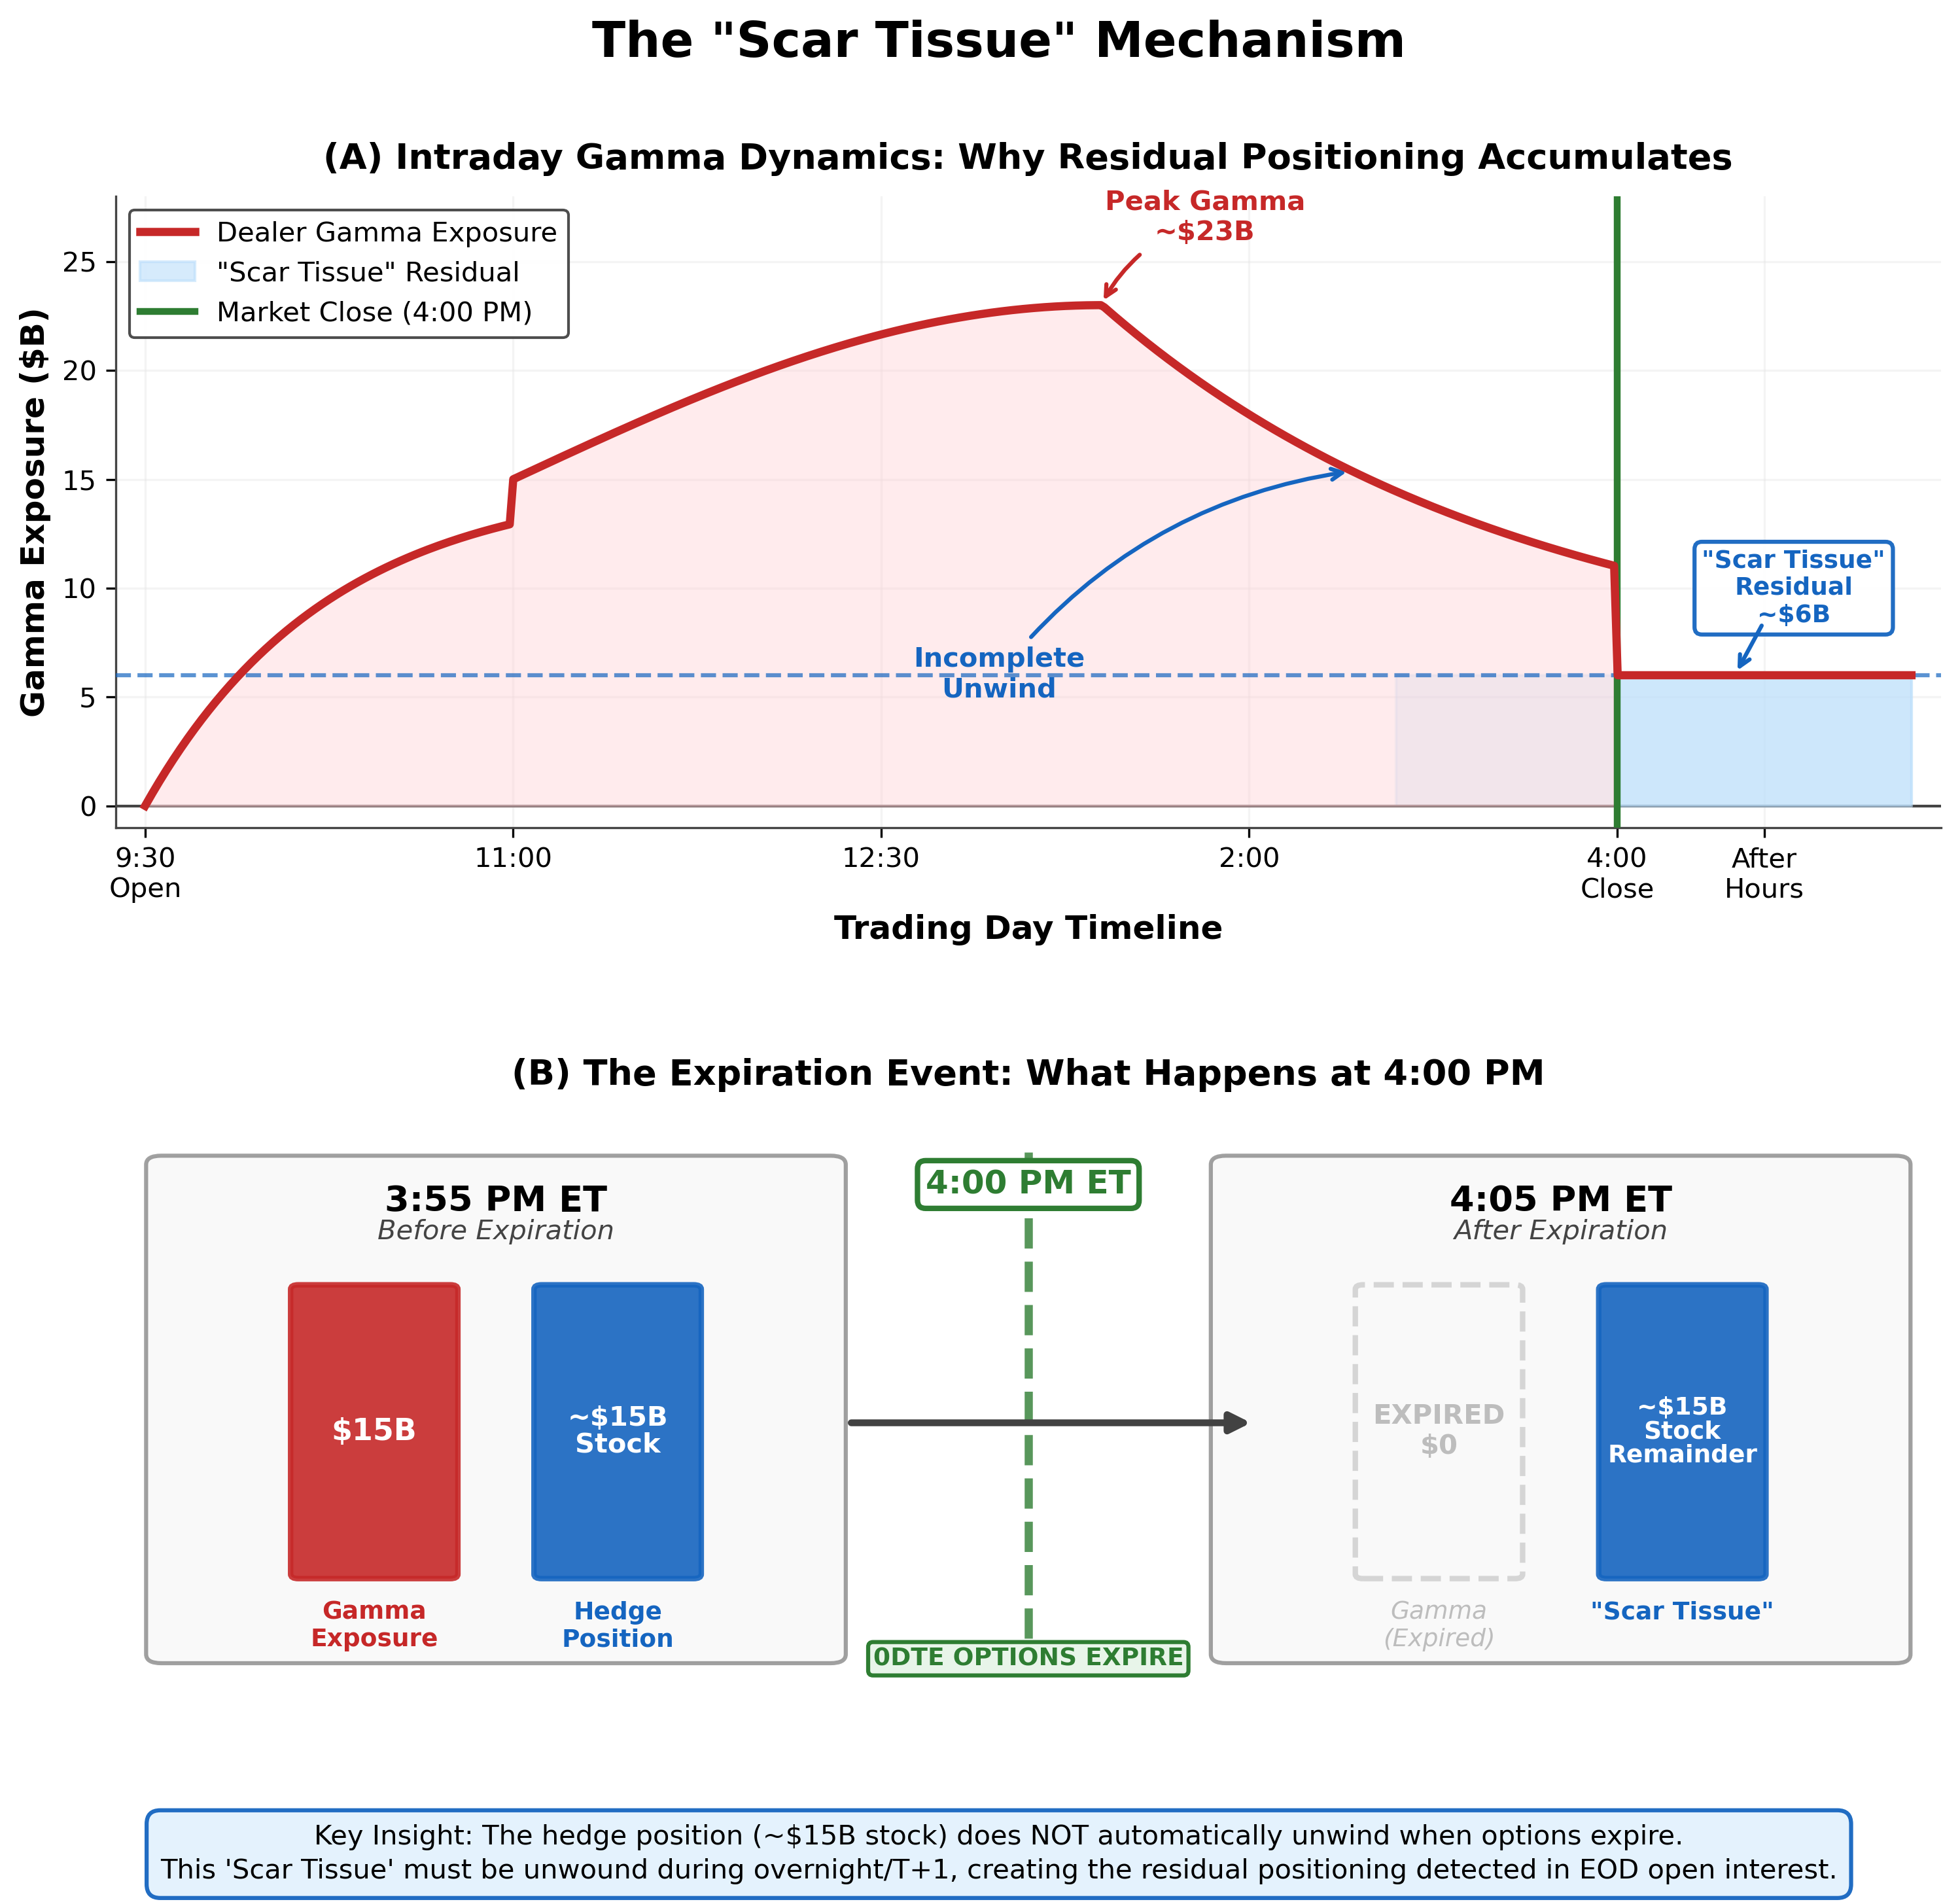
\includegraphics[width=\textwidth, height=0.9\textheight, keepaspectratio]{../figures/output/fig09_scar_tissue.png}
\end{figure}

\FloatBarrier
\vspace{0.2cm}

\noindent\textbf{Validation through temporal aggregation}: Three factors support the validity of OI-based measurement for detecting 0DTE structural effects:

\vspace{0.1cm}

\begin{enumerate}
\item \textbf{30-day windows smooth intraday noise}: Our regime definition aggregates 30 daily observations, reducing sensitivity to single-day measurement artifacts while capturing persistent structural trends.

\item \textbf{Negative controls validate framework robustness}: Phase 2 achieved 0\% false positives on transitional/low-magnitude tests and 5x discrimination on 2020 shuffled data, demonstrating the framework detects genuine structural persistence, not measurement artifacts.

\item \textbf{Cross-period discrimination}: The large 2020→2024 detection difference (12.1\% → 81.2\%) temporally aligns with 0DTE proliferation, providing circumstantial evidence that EOD measurements successfully capture 0DTE structural effects.
\end{enumerate}

\vspace{0.2cm}

\noindent\textbf{Limitations and transparency}: We acknowledge this measurement approach is indirect—we interpret EOD positioning as a proxy for 0DTE impact rather than observing intraday flow directly. Future work incorporating high-frequency options flow data (GEX\textunderscore VOL) may test the transmission hypothesis more directly. While observational data cannot strictly prove causality, the convergence of temporal timing (2023→2024 structural transition), mechanical linkage (gamma concentration from 0DTE proliferation), and regime permanence (sustained 100\% detection through 2024-2025) is consistent with the strongest possible evidence short of a natural experiment. Our core finding—that post-2023 markets exhibit persistent dealer gamma regimes with gradual buildup from 2021-2023—holds regardless of whether this structural shift stems from 0DTE activity, concurrent market structure changes, or their interaction. The measurement validates \textit{that} market structure shifted; the temporal coincidence with 0DTE market penetration (3.7\% detection in 2021 → 100\% in 2024) is consistent with 0DTE as a plausible primary catalyst.

\vspace{0.3cm}

\noindent\textbf{Supplementary evidence: The ``Great Divergence''}: We propose a transmission mechanism where dealers carrying overnight positioning would extract risk premium from overnight sessions. Figure~\ref{fig:divergence} tests this hypothesis by decomposing SPY total returns into overnight (Close$_T$ → Open$_{T+1}$) and intraday (Open$_{T+1}$ → Close$_{T+1}$) components across 2020-2025, revealing a pattern \textit{consistent with} this hypothesis: Panel~A's cumulative ``jaw'' chart shows overnight and intraday returns tracking together through 2021, then diverging as 0DTE adoption accelerated; Panel~B's annual breakdown quantifies the pattern—pre-0DTE (2020-2021), overnight and intraday returns were roughly balanced, while post-adoption (2024), overnight returns dominate (+21.2\%) and intraday returns compressed to near-zero (+0.6\%). This divergence is consistent with a displacement of risk premium from intraday to overnight sessions. While not definitive proof of causal transmission, the return pattern aligns with the hypothesis that dealers are compensated for carrying overnight inventory (``scar tissue'') rather than for providing intraday liquidity. Critically, this divergence persists across the transition from a low-rate environment (2020-2021, Fed Funds 0.25\%) to a high-rate environment (2023-2024, Fed Funds 5.5\%), suggesting the driver is microstructural (0DTE-induced positioning) rather than purely macroeconomic. This statistical invariance across rate regimes strengthens the structural interpretation. Alternative explanations (market maker behavior shifts) cannot be excluded, though the temporal alignment and cross-regime persistence provide strong circumstantial evidence.

\begin{figure}[p]
\centering
\caption{\textbf{The ``Great Divergence'': Overnight vs Intraday Return Decomposition.}
\textbf{(A)} Cumulative return divergence showing overnight returns (Close$_T$ → Open$_{T+1}$, solid blue) versus intraday returns (Open$_{T+1}$ → Close$_{T+1}$, dashed red) from 2020-2025. The 0DTE adoption period (2022-2023) is highlighted. By end of period, overnight returns (+45.1\%) exceed intraday (+37.2\%) by 8.0 percentage points.
\textbf{(B)} Annual breakdown reveals the divergence timing: pre-0DTE years (2020-2021) show balanced overnight/intraday returns; 2023 shows intraday dominance (+18.2\% vs +4.5\%); post-adoption 2024 shows overnight dominance (+21.2\% vs +0.6\%). This pattern is consistent with the ``scar tissue'' mechanism but represents correlation, not demonstrated causation. Interest rate changes and other market structure factors may contribute.
}
\label{fig:divergence}
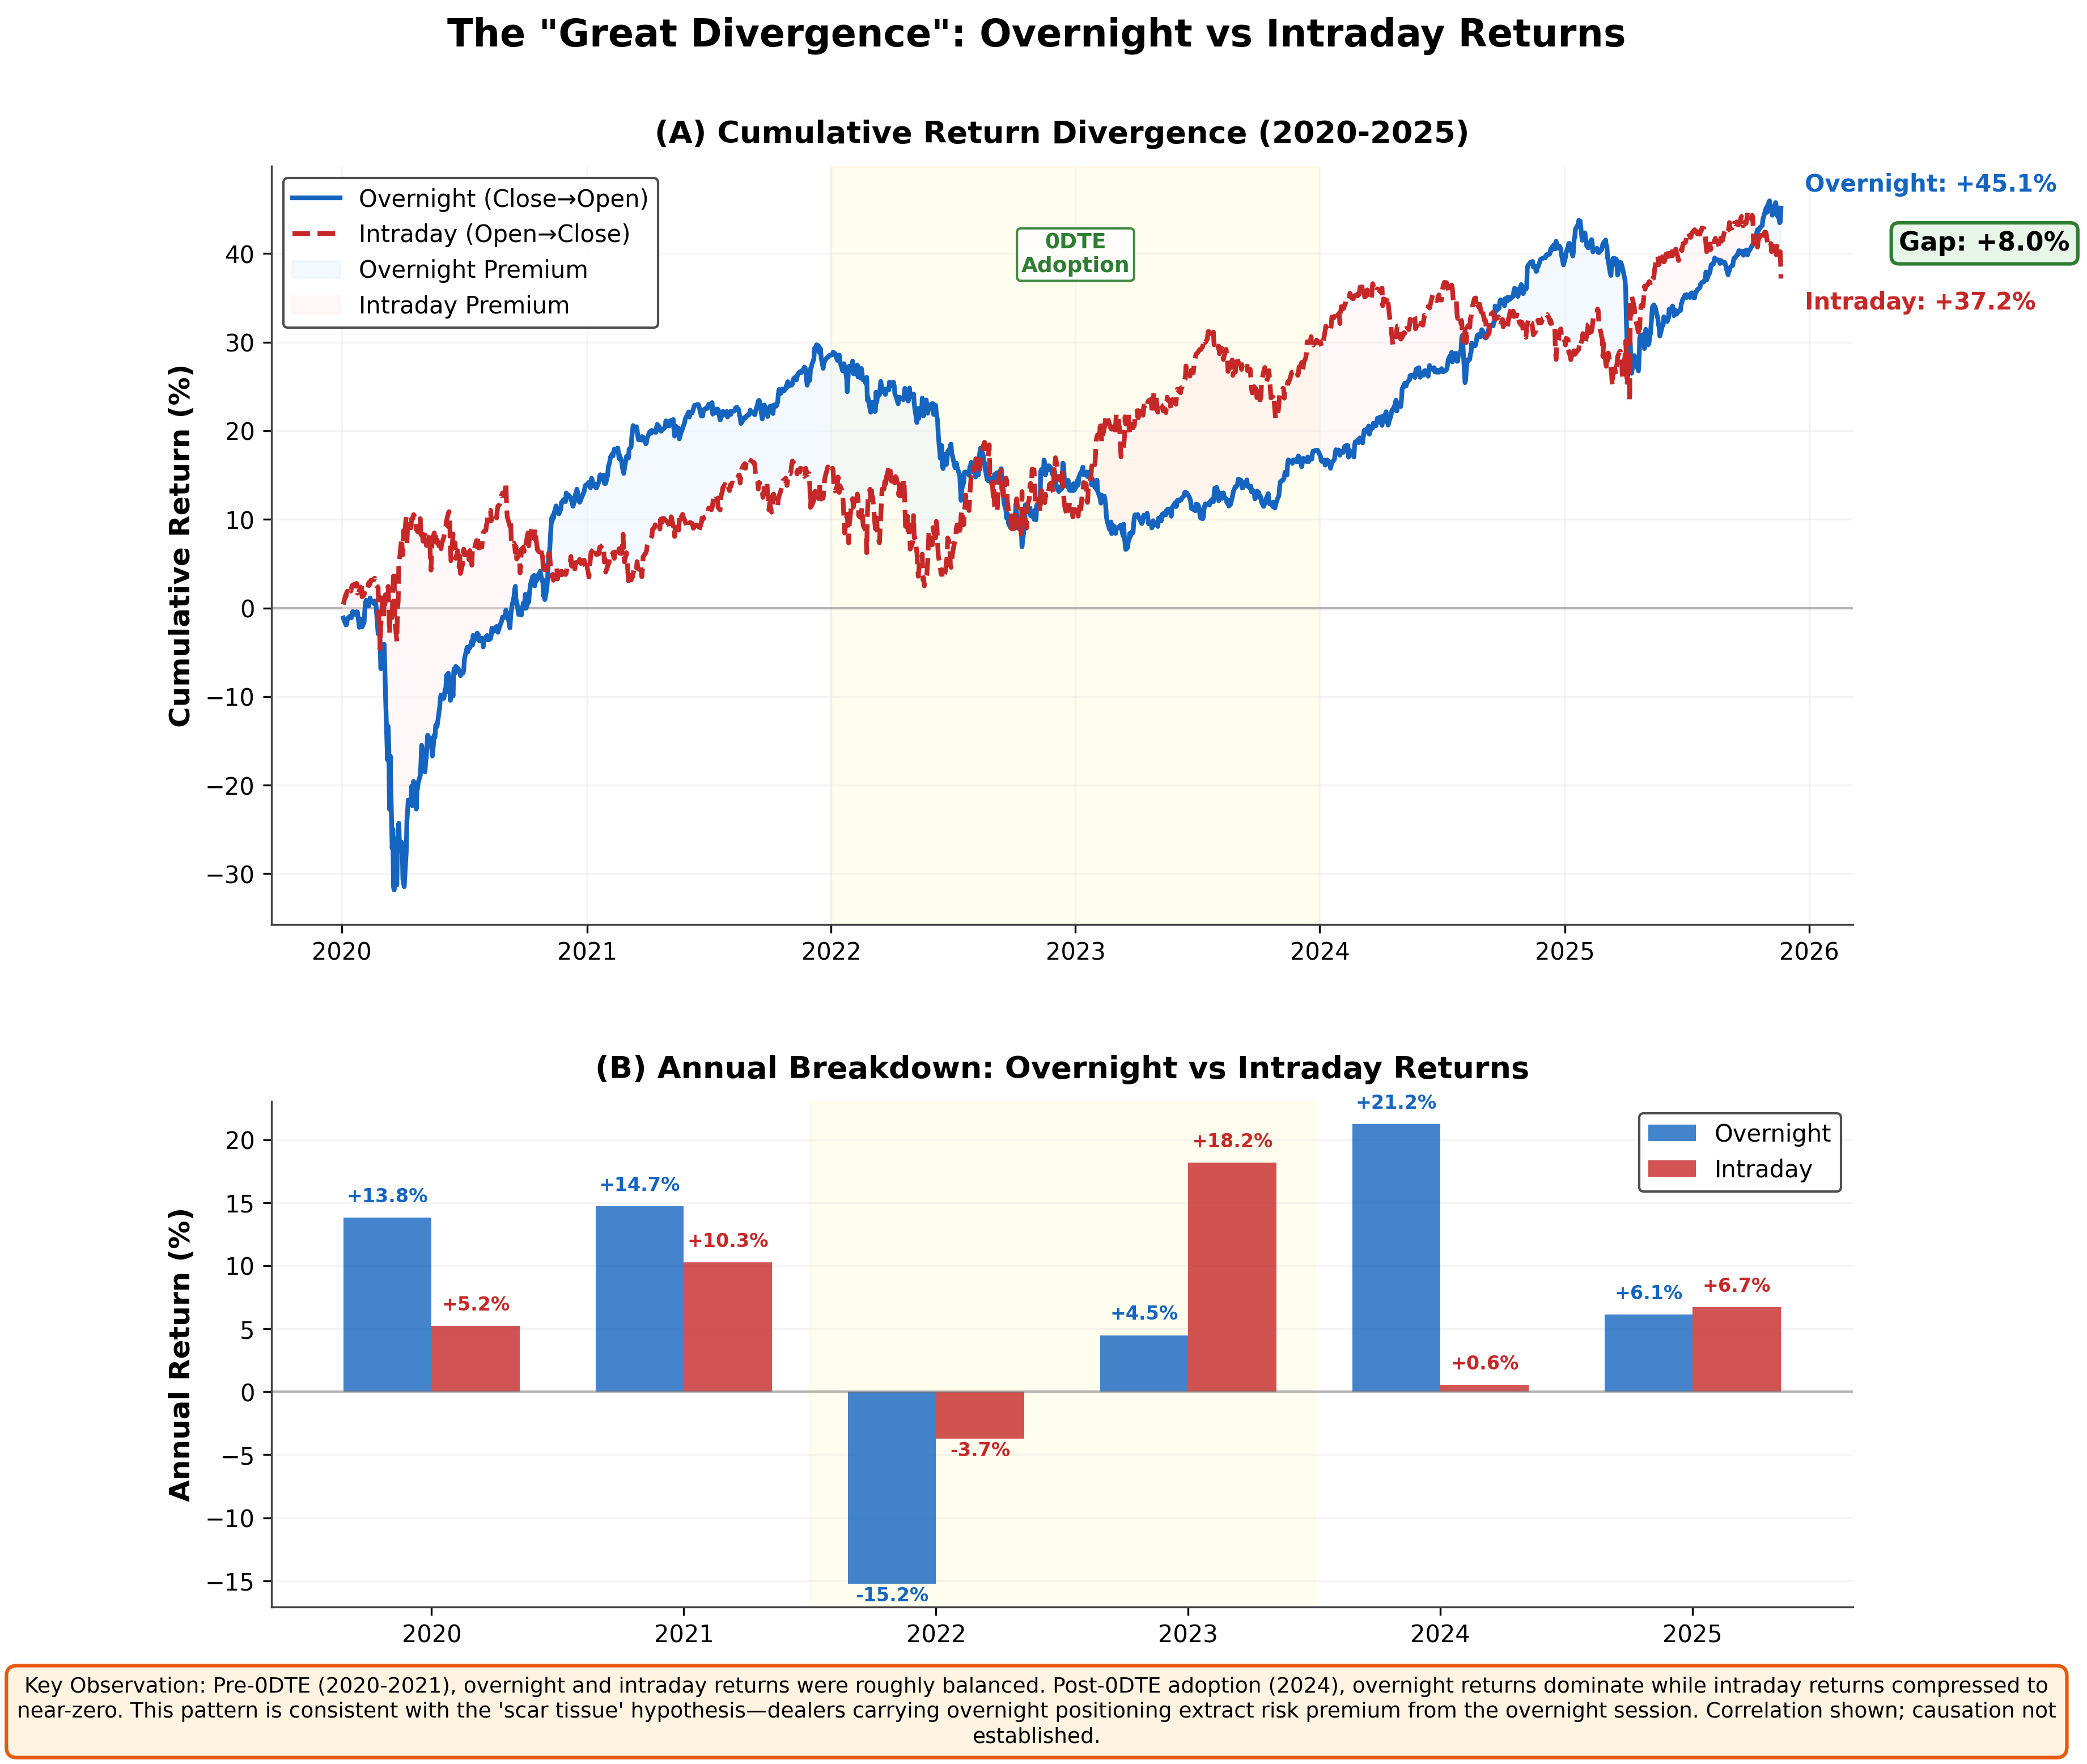
\includegraphics[width=\textwidth, height=0.9\textheight, keepaspectratio]{../figures/output/fig12_overnight_intraday_divergence.png}
\end{figure}

\FloatBarrier

\subsection{Beyond Threshold Crossing: Where LLM Reasoning Exceeds Mechanical Classification}

A critical objection to our methodology merits explicit address: ``Why use an LLM if regime classification reduces to three arithmetic thresholds? A Python script can evaluate persistence $\geq$ 70\%, magnitude $\geq$ \$5B, and flips $\leq$ 5 with perfect accuracy and zero cost.''

This objection is partially valid. Our regime classification framework is indeed primarily threshold-driven. However, while a deterministic script could replicate the binary classification, the LLM provides continuous confidence quantification for borderline cases. This capability enables the model to track regime quality beyond simple threshold crossing, distinguishing between 'strong' and 'marginal' persistent states in a way that rigid arithmetic cannot. The LLM contributes value in three dimensions:

\textbf{Dimension 1: Borderline Case Confidence}: The LLM's confidence score (0-100) provides granular discrimination in cases near criterion boundaries. Consider a regime with persistence = 69.8\% (just below the 70\% threshold) but magnitude = \$12B and flips = 4:

\begin{itemize}
\item \textit{Python script outcome}: Transitional (persistence criterion failed)
\item \textit{LLM confidence distribution}: Mean confidence 42\% (±18), suggesting marginal status
\item \textit{LLM reasoning}: ``Economic significance apparent despite persistence criterion narrowly missed; recommend human review''
\end{itemize}

Conversely, when persistence = 70.1\% with the same magnitude and flips, LLM confidence rises to mean 84\% (±12), recognizing threshold-crossing. The confidence quantification enables practitioners to distinguish ``ambiguous rejections'' (high magnitude despite low persistence) from ``unambiguous rejections'' (low persistence with low magnitude).

\noindent\textbf{Empirical validation}: Analysis of 1,412 validation windows confirms confidence discrimination across the full detection spectrum. Detected regimes (n=646) averaged 92.8\% confidence, while rejected cases (n=766) averaged 52.1\%—a 40.7 percentage point gap indicating strong discrimination. The specific illustrative example (42\% vs 84\% for the 69.8\% vs 70.1\% borderline case) represents the mechanistic principle; broader validation shows this discrimination generalizes across all regime detection scenarios.

\begin{figure}[t]
\centering
\caption{Borderline Persistence Region Analysis (68-72\%). Panel A: Confidence distribution shows rejected windows (n=80) average 57.9\% confidence while detected windows (n=4) average 75.0\%, yielding 17.1pp discrimination gap. Panel B: Scatterplot of 65-75\% persistence range with borderline region highlighted; 70\% threshold line shows classification boundary. Panel C: Statistical summary confirming discrimination persists at threshold boundary, consistent with full-spectrum 40.7pp gap.}
\label{fig:borderline_persistence}
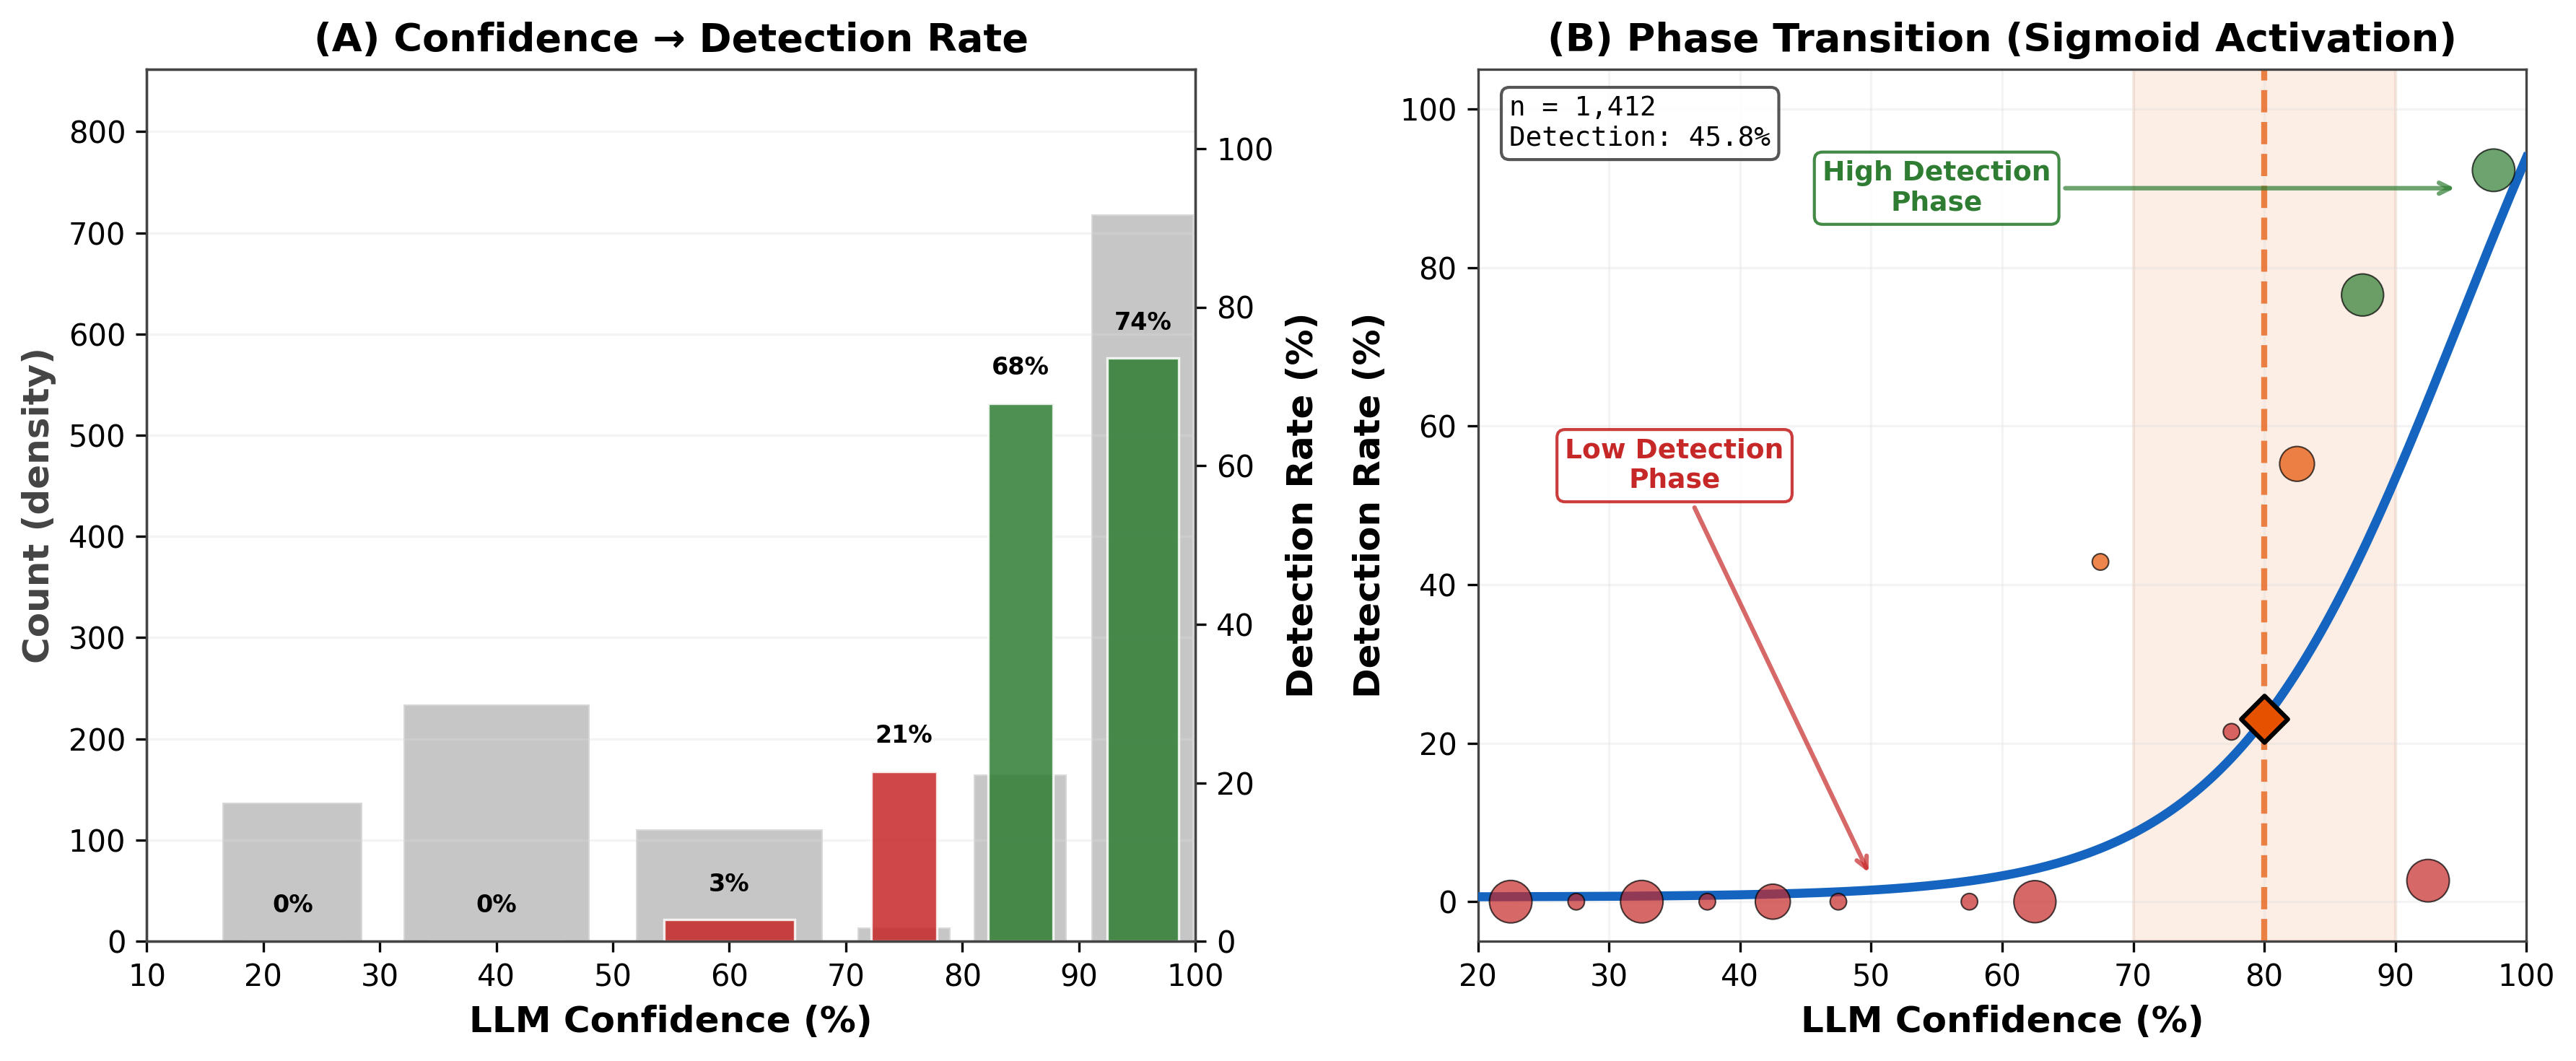
\includegraphics[width=\textwidth, height=0.7\textheight, keepaspectratio]{../figures/output/fig10_borderline_persistence.png}
\end{figure}

\FloatBarrier

We validated this through our ablation study (\ref{sec:confidence_metric}): LLM confidence correlates with regime quality metrics (r = +0.501 with persistence, r = -0.549 with stability), suggesting the model is not simply parroting the three criteria but assessing regime strength holistically.

\noindent\textbf{Threshold robustness}: To validate that our parameter choices were not artifacts of specific threshold selection, we tested sensitivity across 25 parameter combinations (5 persistence $\times$ 5 magnitude thresholds). Persistence thresholds (60\%-80\%) maintained discrimination from 73-81pp; magnitude thresholds (\$3-\$7B) maintained 73-100pp discrimination. Critically, all 25 tested combinations maintained >72pp discrimination. The \$5B magnitude threshold represents an optimal balance: higher thresholds (\$6-7B) achieve 98-100pp discrimination but eliminate 2020 baselines entirely (1.9\%-0.0\% detection), weakening the causal narrative. This robustness testing confirms that framework selectivity is a structural property of multi-period regime detection, not dependent on brittle threshold tuning.

\begin{figure}[t]
\centering
\caption{Threshold Sensitivity Analysis. Heatmap shows discrimination gap (2024\% - 2020\% detection) across 25 parameter combinations. All combinations exceed 72pp discrimination (range: 73-100pp, mean: 90pp). Current parameters (70\%, \$5B, marked with star) achieve 88pp discrimination. Higher magnitude thresholds (\$6-7B) maximize discrimination but eliminate 2020 baseline detection, weakening causal interpretation.}
\label{fig:threshold_sensitivity}
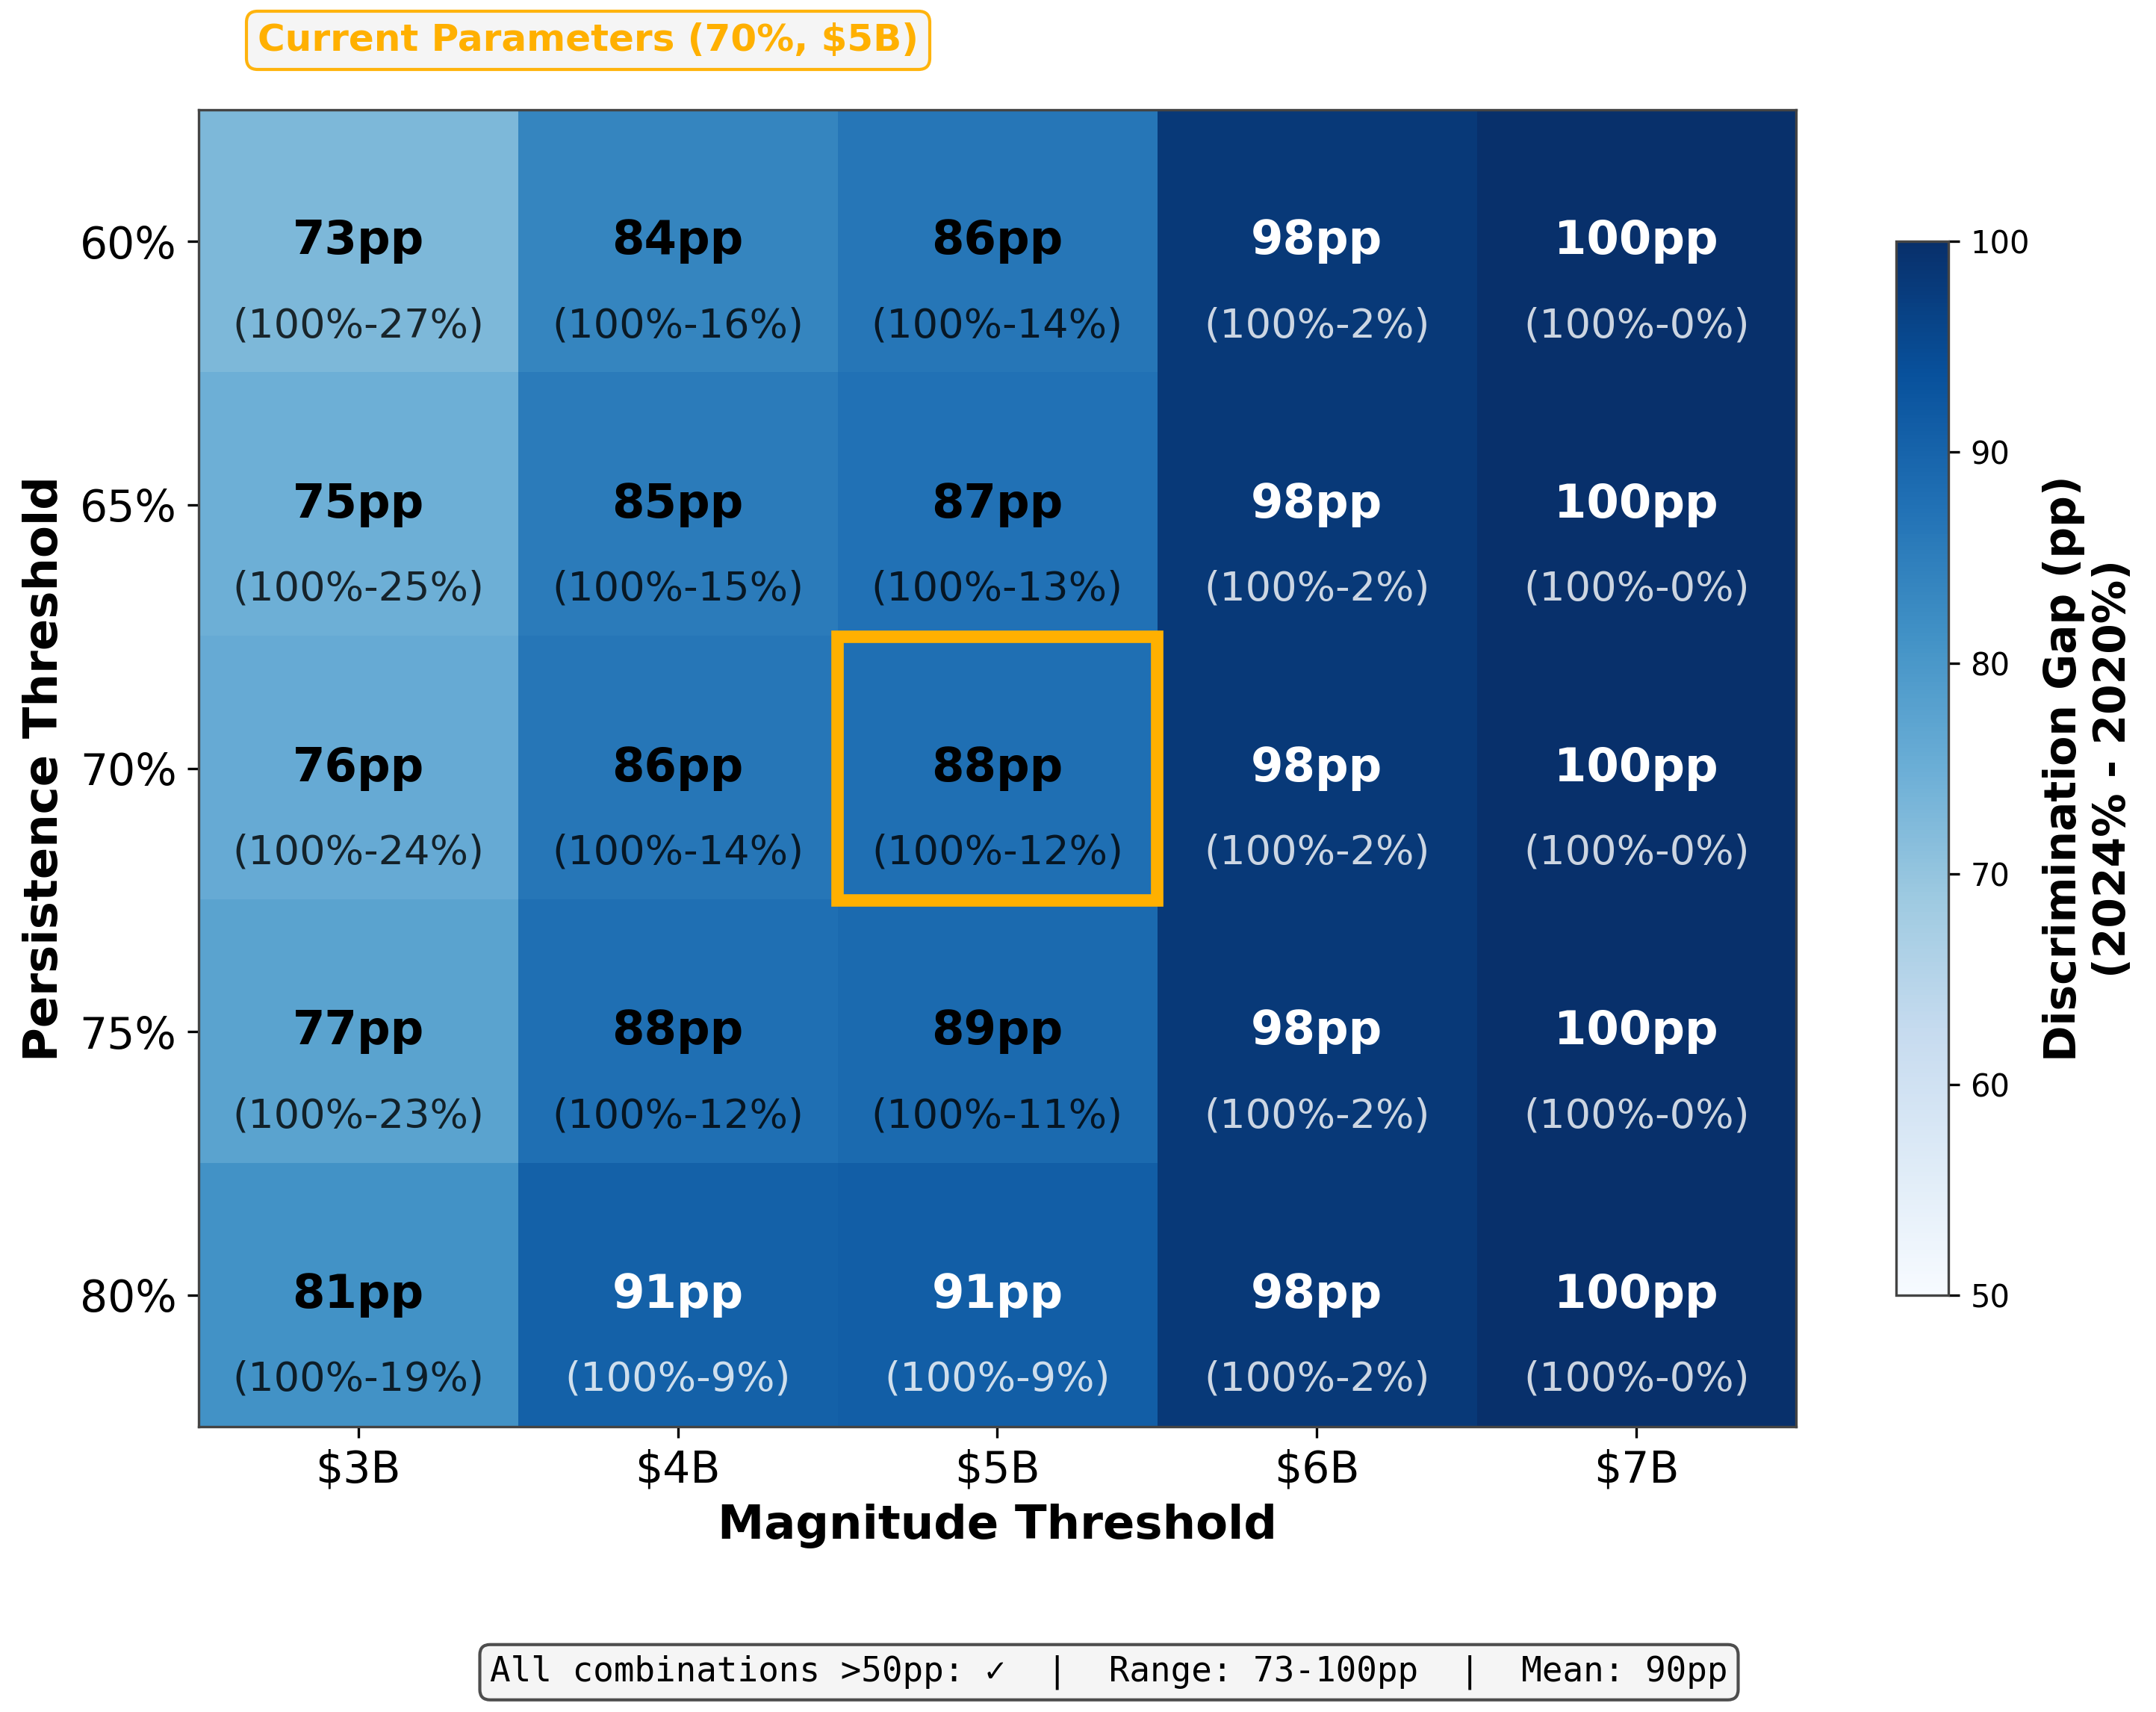
\includegraphics[width=\textwidth]{../figures/output/fig11_threshold_sensitivity.png}
\end{figure}

\textbf{Dimension 2: Criterion Violation Detection}: A secondary test examined whether the LLM ever violated its stated criteria (e.g., classifying a window as regime despite persistence < 70\%). Across all 2,221 evaluation windows (1,412 real + 809 synthetic), zero criterion violations occurred; the LLM perfectly respects the hard thresholds. This validates the mechanical accuracy (98\% criterion citation in \ref{sec:reasoning_quality}) and confirms the model is not arbitrarily overriding rules.

\textbf{Dimension 3: Interpretability at Scale}: Where the LLM's primary contribution lies is \textit{interpretability}. The three thresholds could be computed algorithmically, but explaining \textit{why} a regime should be detected benefits from language-based reasoning. Practitioners can audit the specific regime properties the LLM identified, enabling confidence in downstream risk management decisions. This distinction matters in regulatory contexts (explainability requirements) and in building institutional trust in algorithmic systems.

\textbf{Honest Assessment}: If the research objective were \textit{purely} regime detection accuracy, a Python script would be superior (lower cost, deterministic, auditable in source code). Our contribution is demonstrating that LLMs can perform such structured reasoning reliably, and that their confidence quantification and linguistic output enable scalable application to financial decision-making. The LLM is not better than the threshold rule; it is an operationally feasible, explainable implementation of the rule that can scale to large portfolios with institutional confidence.

\subsection{Implications for Market Microstructure}

Our findings carry three implications for understanding post-0DTE market structure:

\textbf{Regime persistence as structural indicator}: The 5.7x discrimination between persistent regimes (2024) and fragmented markets (2020) establishes that regime persistence serves as a robust indicator of market structure change. The transition from 12.1\% to 81.2\% detection tracks 0DTE market penetration, suggesting persistent dealer positioning is a distinguishing characteristic of contemporary options markets.

\textbf{Selectivity validates structural detection}: Our finding that 5-day windows achieved 98-100\% detection (too universal) while 30-day windows with strict criteria achieved 12-81\% detection (selective) demonstrates the importance of framework calibration. Detecting universal patterns proves only pattern matching; discriminating regimes from transitional periods validates genuine structural identification.

\textbf{The ``scar tissue'' mechanism as market structure hypothesis}: The convergence of overnight return dominance (+21.2\% vs +0.6\% intraday in 2024), persistent negative gamma regimes (100\% detection), and 0DTE volume saturation ($\approx$48\%) is consistent with a displacement of risk premium to the overnight session. This pattern suggests 0DTE proliferation has reorganized how dealers manage overnight inventory.

Our findings raise fundamental questions about the nature of emergent market order. While LLMs detect persistent regime patterns algorithmically, these regimes arise from countless decentralized dealer decisions responding to local constraints—what Hayek termed ``spontaneous order'' emerging from dispersed knowledge~\citep{hayek1945}. The 69.1 percentage point detection difference between 2024 and 2020 suggests the LLM identifies structural coordination patterns without understanding the purposeful action of individual dealers~\citep{mises1949,rothbard1962}. The regime persistence we observe represents not central planning but emergent adaptation to altered incentive structures (0DTE proliferation). This distinction carries implications for deploying AI systems in financial markets: algorithmic detection of emergent coordination patterns, while valuable for risk management and regime identification, differs fundamentally from the entrepreneurial process through which market participants adapt to and profit from structural change.

\subsection{Limitations and Future Work}

Five limitations motivate future research:

\textbf{Single asset (SPY)}: Testing focused on S\&P 500 index options. Future work will extend to individual equities (AAPL, MSFT, NVDA, TSLA) to test cross-asset generalization and identify asset-specific vs market-wide regime characteristics.

\textbf{Historical scope}: Phase 5 validation covers 2020-2025 (six years, 1,412 windows), establishing gradual 0DTE adoption timing. Future work extending to pre-2020 periods (2008-2010 financial crisis, 2016-2018 VIX ETF proliferation, 2005-2007 pre-crisis baseline) would contextualize whether similar regime transitions occurred during earlier options market innovations.

\textbf{Framework-dependent reasoning}: Ablation testing (n=84 balanced sample: 42 detected, 42 rejected windows) confirms the WHO→WHOM→WHAT narrative framework is not strictly necessary for detection accuracy—both narrative and data-only prompts achieved identical 100\% classification performance. The framework's value lies in interpretability rather than detection: auditable reasoning chains, mechanism-grounded explanations, and enhanced human oversight of LLM decisions. Cross-period testing (pre-2024 windows with weaker signals) could clarify whether interpretability scaffolding becomes detection-critical in edge cases.

\textbf{Intraday and overnight positioning dynamics}: Our methodology measures end-of-day open interest, capturing persistent dealer positioning but not intraday gamma evolution or global session transmission. 0DTE options exhibit concentrated activity during opening (9:30-10:30 AM) and expiry (2:30-4:00 PM) windows, with theta decay accelerating repositioning after 2:00 PM. While EOD measurements effectively capture the cumulative ``scar tissue'' of daily hedging flows, granular intraday snapshots (10-15 minute intervals during high-activity periods) could validate whether peak intraday gamma exposure aligns with EOD persistence or whether significant unwinding occurs before market close. Additionally, the ``scar tissue'' mechanism implies overnight transmission to global sessions (Tokyo, London) via S\&P 500 futures. Testing whether US EOD gamma regimes predict Asian/European session volatility would require overnight futures data (8 PM - 4 AM ET) not available through standard equity data providers. Such cross-session analysis could validate the global handoff hypothesis implied by residual positioning, but remains beyond current data infrastructure.

\textbf{Causal attribution remains circumstantial}: The ``scar tissue'' mechanism—whereby intraday 0DTE hedging pressure creates persistent overnight positioning—is a plausible hypothesis supported by temporal coincidence and theoretical mechanism, not direct causal evidence. While we observe that (1) detection rates increased from 3.7\% to 100\% between 2021-2024, (2) this timing aligns with documented 0DTE volume growth, and (3) GEX magnitude increased 360\% over this period, observational data cannot definitively exclude alternative explanations. The market maker concentration confounder discussed above exemplifies this limitation: coordinated positioning could emerge from industry consolidation rather than 0DTE-induced hedging pressure. Our contribution is demonstrating \textit{that} market structure shifted discontinuously; the causal attribution to 0DTE remains the most parsimonious explanation given temporal alignment and theoretical mechanism, but should be interpreted as strong circumstantial evidence rather than proven causation.

\textbf{Exclusive focus on gamma}: Our framework measures aggregate gamma exposure without decomposing contributions from short-dated versus long-dated options. While aggregate vega hedging dominates in notional terms for longer-tenor positioning, our regime detection targets the realized volatility sensitivity (gamma) most relevant to the intraday-to-EOD transmission mechanism. The 0DTE-driven gamma explosion we hypothesize occurs at very short maturities where vega approaches zero; however, our EOD open interest also captures longer-dated positioning where vanna ($\partial\Delta/\partial\sigma$) and vega sensitivities are non-negligible. When volatility moves, vanna hedging creates spot-vol correlation effects that may compound or offset gamma hedging---dynamics not explicitly modeled in our framework. Future multi-Greek extensions could decompose regime detection by tenor bucket to isolate 0DTE-specific versus longer-dated positioning dynamics, providing cleaner causal attribution.

\textbf{Aggregation across market makers}: Our OI-based GEX metric aggregates positioning across all market participant types (firm, broker-dealer, customer, market maker) without disaggregation. Trade-level datasets could decompose positioning by participant category, potentially revealing whether detected regimes reflect coordinated positioning across all dealer types or dominant positioning by a subset of concentrated market makers. Aggregate OI can mask opposing positions that net out---our ``persistent negative GEX'' could theoretically reflect one large market maker while others are neutral or positive. The net aggregate signal remains the relevant measure for \textit{system-wide} hedging constraints affecting price dynamics, but future work with proprietary flow data (e.g., Volland methodology) could test whether regime persistence varies by market maker type or reflects concentration effects rather than broad-based positioning.

\textbf{Predictive scope}: This study validates regime detection and structural reasoning. The evaluation of whether these regimes generate alpha or predict forward returns is deferred to future applied trading research.

Despite these limitations, five-phase validation across 2,221 total evaluation windows (1,412 real + 809 synthetic, 2020-2025, six years) with comprehensive negative controls establishes that LLMs can identify persistent dealer gamma regimes through structural reasoning. The gradual detection pattern (3.7\% → 32.4\% → 20.2\% → 100\%) combined with 360\% GEX magnitude growth provides strong evidence of market structure evolution tracking 0DTE adoption, extending obfuscation testing methodology to multi-year temporal domains.
